\documentclass{article}

% Packages for code listing and syntax highlighting
\usepackage{listings}
\usepackage{xcolor}
\usepackage[margin=3cm]{geometry} % Adjust the margin value as desired
\usepackage{setspace}
\usepackage{tikz}
\usepackage{graphicx}
\usepackage{float}
\usepackage{textcomp}
\usepackage{multicol}
\usepackage{enumitem}

\onehalfspacing

% Define the color theme
\definecolor{codebackground}{RGB}{242, 242, 242}
\definecolor{codekeyword}{RGB}{0, 0, 255}
\definecolor{codecomment}{RGB}{63, 127, 95}
\definecolor{codestring}{RGB}{163, 21, 21}

% Code listing style for all languages
\lstdefinestyle{mystyle}{
    backgroundcolor=\color{codebackground},
    basicstyle=\footnotesize\ttfamily,
    keywordstyle=\color{codekeyword}\bfseries,
    commentstyle=\color{codecomment}\itshape,
    stringstyle=\color{codestring},
    numbers=left,
    numberstyle=\tiny\color{codecomment},
    stepnumber=1,
    numbersep=8pt,
    showstringspaces=false,
    breaklines=true,
    frame=single,
    frameround=none,
    framesep=5pt,
    rulecolor=\color{codebackground},
    tabsize=4,
    captionpos=b,
    xleftmargin=15pt,
    xrightmargin=15pt
}

% Set the default style for code listings
\lstset{style=mystyle}

% Additional packages and settings for math typesetting
\usepackage{amsmath}
\usepackage{amssymb}
\usepackage{bm}

% Define your document content
\begin{document}

\title{Numbering Systems and Base Encoding}
\author{Abyan Majid}
\date{July 5, 2023}
\maketitle

\section{Numbering systems typically found in computer systems}

There are 4 different numbering sytems that are typically found in computer systems:

\begin{itemize}
    \item Decimal (base 10): Decimal numbers may ONLY be represented by the values [0, 1, 2, 3, 4, 5, 6, 7, 8, 9]
    \item Binary (base 2): Binary numbers may ONLY be represented by the values [0 and 1].
    \item Octal (base 8): Octal numbers may ONLY be represented by the values [0, 1, 2, 3, 4, 5, 6, 7]
    \item Hexadecimal (base 16): Hexadecimal numbers may ONLY be represented by the values [0, 1, 2, 3, 4, 5, 6, 7, 8, 9, A, B, C, D, E, F]
\end{itemize}

\begin{center}
    Decimals are what we humans currently use to count. Binaries are what computers use. Octal and hexadecimals are useful abbreviations for binaries because they're often lengthy.
\end{center}

\noindent\hrulefill

\noindent For example, the decimal number 25 can also be represented as:

\begin{itemize}
    \item "11001", on base 2 (binary). Or, we write "\underline{0b}11001" to clearly indicate that it is a binary.
    \item "31", on base 8 (octal). Or, we write "\underline{0o}31" to clearly indicate that it is an octal.
    \item "19", on base 16 (hexadecimal). Or, we write "\underline{0x}19" to clearly indicate that it is a hexadecimal.
\end{itemize}

\section{Base encoding}
In this section, we will explore ways to represent a number, with the example of 25, in base 10, 2, 8, and 16.
\subsection{Translating base 10 to base 2 (decimal to binary)}

You can convert from base 10 to base 2 (ie decimal to binary) through successive division.
$$\frac{25}{2}=12\times2+\fbox{1}\phantom{1}\text{(least significant bit)}$$
$$\frac{12}{2}=6\times2+\fbox{0}$$
$$\frac{6}{2}=3\times2+\fbox{0}$$
$$\frac{3}{2}=1\times2+\fbox{1}$$
$$\frac{1}{2}=0\times2+\fbox{1}\phantom{1}\text{(most significant bit)}$$

\vspace{\baselineskip}
\noindent What happened here is we kept on dividing by 2 until we no longer can. However, each time we divide by 2, we do not write literal decimals but rather in quotient and remainder format.

\begin{center}
    IMPORTANT: The REVERSE order of the remainders is the binary or base 2 representation of the decimal. So, in this case, the binary or base 2 representation of the decimal "25" is \fbox{11001}, otherwise written as "0b11001".
\end{center}

\subsection{Translating base 2 to 10 (binary to decimal)}
To convert from base 2 to base 10 (ie binary to decimal) you multiply each bit by $2^n$, where $n$ is the position of the bit in the binary - starting from the last, rightmost bit, in which case $n=0$.

\begin{center}
So, basically, you perform \fbox{$b\times2^n$} starting from the rightmost bit until the leftmost. $n$ should start at 0 and increments by 1 with every next bit. \\
\vspace{\baselineskip}
\begin{tikzpicture}[->,>=stealth,thick]
    % Nodes
    \node (d4) at (0,0) {1};
    \node (d3) at (2,0) {1};
    \node (d2) at (4,0) {0};
    \node (d1) at (6,0) {0};
    \node (d0) at (8,0) {1};
    
    % Binary digits
    \node (b4) at (0,-2) {$1\times2^4$};
    \node (b3) at (2,-2) {$1\times2^3$};
    \node (b2) at (4,-2) {$0\times2^2$};
    \node (b1) at (6,-2) {$0\times2^1$};
    \node (b0) at (8,-2) {$1\times2^0$};
    
    % Calculation
    \node (c4) at (0,-4) {16};
    \node (c3) at (2,-4) {8};
    \node (c2) at (4,-4) {0};
    \node (c1) at (6,-4) {0};
    \node (c0) at (8,-4) {1};
    
    % Arrows
    \draw (b4) -- (c4);
    \draw (b3) -- (c3);
    \draw (b2) -- (c2);
    \draw (b1) -- (c1);
    \draw (b0) -- (c0);
    
    \draw (d4) -- (b4);
    \draw (d3) -- (b3);
    \draw (d2) -- (b2);
    \draw (d1) -- (b1);
    \draw (d0) -- (b0);
  \end{tikzpicture}
  
  \vspace{\baselineskip}
  The sum gives the decimal or base 10 representation. \\
  \vspace{\baselineskip}
  $16+8+0+0+1=\fbox{25}$
\end{center}

\subsection{Translating base 2 to base 8 (binary to octal)}
When converting base 2 to base 8 (ie binary to octal), we group the binary into sets of 3, starting from the right. We do this because $2^3$ (which is 8) is the common factor between the binary and octal number system.

\begin{center}
    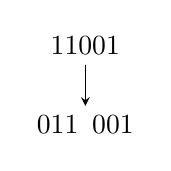
\begin{tikzpicture}[->,>=stealth]
        % Nodes
        \node (b1) at (4,0) {11001};
        
        % Binary digits
        \node (b2) at (4,-1) {$011\phantom{2}001$};
        
        % Arrows
        \draw (b1) -- (b2);
      \end{tikzpicture} \\
    If a set has fewer than 3 bits, we add a prefix of leading zeros (e.g. $11\rightarrow011$). \\
    \vspace{\baselineskip}
    Next, we get the corresponding octal value for each set of 3 bits. \\
    \vspace{\baselineskip}
    \begin{tabular}{|c|c|}
        \hline
        \textbf{3-bit Binary} & \textbf{Octal} \\
        \hline
        000 & 0 \\
        \fbox{001} & \fbox{1} \\
        010 & 2 \\
        \fbox{011} & \fbox{3} \\
        100 & 4 \\
        101 & 5 \\
        110 & 6 \\
        111 & 7 \\
        \hline
    \end{tabular} \\
    \vspace{\baselineskip}
    So, the octal representation of the binary 11001 is \fbox{31}, otherwise written as "0o31".
\end{center}

\subsection{Translating base 2 to 16 (binary to hexadecimal)}
To convert base 2 to base 16 (ie binary to hexadecimal), you do the same as you would when converting base 2 to base 8.
Except, in this case, you group the binary into sets of 4 bits instead because $2^4$ (which is 16) is the common factor between the binary
and hexadecimal systems.
\begin{center}
    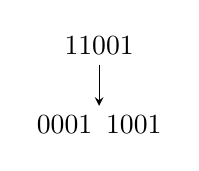
\begin{tikzpicture}[->,>=stealth]
        % Nodes
        \node (b1) at (4,0) {11001};
        
        % Binary digits
        \node (b2) at (4,-1) {$0001\phantom{2}1001$};
        
        % Arrows
        \draw (b1) -- (b2);
      \end{tikzpicture} \\
      Don't forget to add leading zeros as a prefix to sets with less than 4 bits (eg $1\rightarrow0001$) \\
      Now, we get the corresponding hexadecimal digits. \\
      \vspace{\baselineskip}
\begin{tabular}{|c|c|}
    \hline
    \textbf{4-bit Binary} & \textbf{Hexadecimal} \\
    \hline
    0000 & 0 \\
    \fbox{0001} & \fbox{1} \\
    0010 & 2 \\
    0011 & 3 \\
    0100 & 4 \\
    0101 & 5 \\
    0110 & 6 \\
    0111 & 7 \\
    1000 & 8 \\
    \fbox{1001} & \fbox{9} \\
    1010 & A \\
    1011 & B \\
    1100 & C \\
    1101 & D \\
    1110 & E \\
    1111 & F \\
    \hline
\end{tabular} \\
\vspace{\baselineskip}
So, the base 16 or hexadecimal representation of the binary 11001 is \fbox{19}, otherwise written as "0x19"
\end{center}

\subsection{Translating base 8 and 16 to base 2 (octal and hexadecimal to binary)}
This should be self-explanatory, all you have to do is find the corresponding set of bits for each digit in the octal or hexadecimal form.

\begin{itemize}
    \item Octal number "0o31" to binary \\
    - "3" is "011" in binary \\
    - "1" is "001" in binary \\
    Therefore, the binary of "0o31" is \fbox{11001}, with the leading extra zeros "\underline{0}11001" removed.
    \item Hexadecimal number "19" to hexadecimal \\
    - "1" is "0001" in binary \\
    - "9" is "1001" in binary \\
    Therefore, the binary of "0x19" is \fbox{11001}, with the leading extra zeros "\underline{000}11001" removed.
\end{itemize}

\begin{center}
    Refer to the binary to the octal/hexadecimal tables above for reference.
\end{center}

\end{document}